\chapter{Single Qubit Gates}

In this section we will deal with single qubit gates and different ways we can represent them.

A single qubit gate can be represented as an unitary operator acting on the state vector of the qubit.That is for every gate $G$ there exists a unitary transformation $U$ such that the final state of a state vector $\ket{\psi}$ is given by 
$$ \ket{\psi_2} = U\ket{\psi}$$
This is because the gate can be thought of as an abstract machine that takes in a state vector and operates on it with time. As all time transformations of quantum state vectors are unitary transformations the above result holds. Conversely we assume that for every unitary operator on a single qubit there exists a gate for the same. Achieving the construction of such a gate would venture into physical realisation of quantum computation which we reserve for later.

\begin{exercise}
Mathematically prove that all single gate qubit operators have to be unitary by using the normalisation condition of qubit state vectors.
\end{exercise}
\begin{figure}[htp]
    \centering
    \caption{Bloch Representation of a Qubit}
    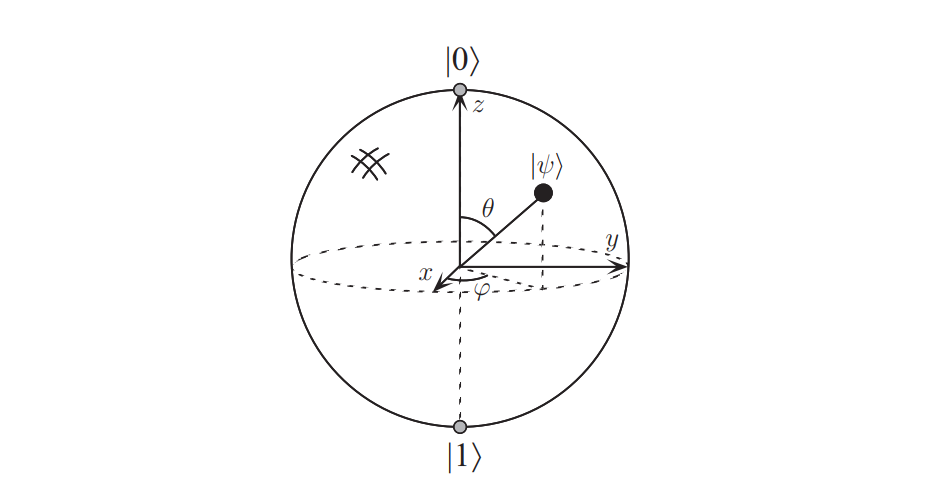
\includegraphics[width=\textwidth]{bloch}
\end{figure}

We now introduce the bloch sphere notation for qubits. Observe that we can write any qubit as follows:
$$\ket{\psi} = e^{ix}\left(\cos{\frac{\theta}{2}} + ie^{i\phi}\sin{\frac{\theta}{2}}\right)$$ where $$ 0 \leq x < 2\pi,   0 \leq \theta \leq \pi,   0\leq \phi <2\pi$$
\\
The global phase $e^{ix}$ is irrelevant as it is common to both. Observe that by neglecting this our state vector is parameterised by $\theta$ and $\phi$ and these values are precisely in the range of the spherical angular coordinates of a sphere of radius 1. Thus corresponding to every $\ket{\psi}\left(\theta, \phi \right)$ there exists a point on the unit sphere given by $(1, \theta, \phi)$ in spherical polar coordinates.
This sphere is termed as the bloch sphere and the corresponding position vector the bloch vector.

It is interesting to note that any unitary transformation in the state space can be visualised to be a rotation of the bloch sphere about an axis. That is this mapping corresponds to a rotation of the bloch sphere (upto a global phase). You will prove this result later on.
We first define some standard gates in their matrix forms. These gates are incredibly useful and are known as the pauli matrices.

$$X = \begin{bmatrix}0&1\\1&0\end{bmatrix}& Y = \begin{bmatrix}0&-i\\i&0\end{bmatrix}&Z=\begin{bmatrix}1&0\\0&-1\end{bmatrix}$$\\

First we would like to describe some standard transformations (or gates) that rotate the sphere about x, y, z axes.

$$R_x(\theta) = e^{-i\theta\frac{X}{2}} = \begin{bmatrix}\cos{\frac{\theta}{2}}& -i\sin{\frac{\theta}{2}}\\-i\sin{\frac{\theta}{2}}&\cos{\frac{\theta}{2}}\end{bmatrix}$$
$$R_y(\theta) = e^{-i\theta\frac{Y}{2}} = \begin{bmatrix}\cos{\frac{\theta}{2}}& -\sin{\frac{\theta}{2}}\\\sin{\frac{\theta}{2}}&\cos{\frac{\theta}{2}}\end{bmatrix}$$
$$R_z(\theta) = e^{-i\theta\frac{Z}{2}} = \begin{bmatrix}e^{\frac{-i\theta}{2}}& 0\\0&e^{i\frac{\theta}{2}}\end{bmatrix}$$

\begin{exercise}
Show that $X^2 = Y^2 = Z^2 = I$ and hence deduce the expansion of their exponentiation as done above using the result of exercise 2.5
\end{exercise}

It is a bit lengthy to show that the above matrices indeed do what we are claiming them to do. You can refer to this \href{http://www.vcpc.univie.ac.at/~ian/hotlist/qc/talks/bloch-sphere-rotations.pdf}{resource} for more detail (you will need to go through density matrices that we introduce in the next section).

It is important to note that in the bloch sphere representation the coefficient along $\ket{0}$ is always a real positive number. After we apply any gate on the state vector this may not be true and so we must first divide by a common phase factor to ensure the above condition is met before we figure out the bloch vector.  

We prove this important theorem that relates unitary transformations to rotation transformations using the rotation matrices.

\begin{theorem}
Suppose U is a unitary transformation. Then there exists reals $\alpha, \beta, \gamma$ and $\delta$ such that 
$$ U = e^{i\alpha}R_z(\beta)R_y(\gamma)R_z(\delta)$$
\end{theorem}

\begin{proof}
Since U is unitary, the rows and columns of U are orthonormal. Thus there exist reals $\alpha, \beta, \gamma$ and $\delta$ such that 
$$U = \begin{bmatrix}e^{i(\alpha - \frac{\beta}{2} - \frac{\delta}{2})}\cos{\frac{\delta}{2}} & -e^{i(\alpha - \frac{\beta}{2} + \frac{\delta}{2})}\sin{\frac{\delta}{2}} \\e^{i(\alpha + \frac{\beta}{2} - \frac{\delta}{2})}\sin{\frac{\delta}{2}}& e^{i(\alpha + \frac{\beta}{2} + \frac{\delta}{2})}\cos{\frac{\delta}{2}}
\end{bmatrix}
$$
By expanding the right hand side of the statement to prove we immediately get the above and thus the given statement is proved.
\end{proof}

The above theorem allows us to construct any gate using just three parameterised gates. There exists an important corollary of the above that we leave as an exercise. This corollary is useful when we want to construct multi qubit gates.

\begin{exercise}
Suppose $U$ is a unitary gate. Show that there exists unitary operators$A, B, C$ on a single qubit such that $ABC=I$ and $U$ is identical to $AXBXC$ upto a global phase.
\end{exercise}

We end this section by mentioning two other important gates that we will later use.
The Hadamard gate was previously introduced and is given by 
$$H = \frac{1}{\sqrt{2}}\begin{bmatrix}1 & 1 \\ 1&-1 \end{bmatrix} $$
The T gate (also known as the $\frac{\pi}{8}$ gate) is given by 
$$ T = \exp(i\pi/8)\begin{bmatrix} \exp(-i\pi/8) & 0 \\ 0 & \exp(i\pi/8) \end{bmatrix}$$

We will revisit quantum gates in detail later. First let us look into composition of quantum systems and tensor products as we will require this when dealing with multi qubit gates.

\clearpage